\section{Discussion}
\label{sec:Discussion}
% Our claims
We find that competition close to neutrality significantly increases the chances of chaotic behaviour. This peak in chaotic dynamics indeed coincided with a peak in biodiversity. These observations, suggest that the hypothesis of non-equilibrium \citep{Huisman1999} and Hubbell's hypothesis of neutrality are not completely independent (see figure \ref{fig:GapInKnowledge}). Additionally we observed that also non-chaotic periodic dynamics  led to a higher biodiversity than stable equilibria.

%% Limitations
Our result seemed to be robust against changes in the number of species. However, the probability of chaotic dynamics is dependent on the model details and all parameters \citep{Dakos2009b}. We explored the variation away from neutrality only by changing the competition strength. We didn't use Allee effects, nor noise, nor species-specific carrying capacities, and the functional form of each term has been chosen to account for satiation and saturation in the simplest possible ways. This opens the door to perform similar analyses in the future using more sophisticated models.

Both the competition and predation parameter sets were drawn from probability distributions. The interactions in our system can be interpreted as a weighted network with a high connectivity. In nature, trophic networks tend to show modular structure with various clusters \citep{Thebault2010}. Our simplified model could be interpreted as representing one of those densely connected modules. Moreover, while in the present paper our random parameters were drawn independently, the competition matrix can be chosen in a more advanced way (for instance, accounting for rock-paper-scissors competition). Studying the effect of different physiological scenarios (in the sense of \citet{Huisman2001}, that is, constrains between the parameters) on the probabilities of chaos could be a continuation to this paper.

% Chaos detection
Due to the large number of simulations made, we had to rely on automatic methods for detecting chaos. Automatic detection of chaos by numerical methods has fundamental limitations, especially for high dimensional systems like ours. Most of them can be boiled down to the fact that, in general, numerical methods cannot distinguish robustly between long, complicated transients and genuine chaos. Our motivation to choose the Gottwald - Melbourne test \citep{Gottwald2009} was threefold: it discriminates between stable, cyclic and chaotic, it escalates easily to systems of higher dimensions, its computation is fast and it performs better than any other method we tried when compared to the visual inspection of the time series. Although we cannot exclude that we misinterpreted some of the generated time series due to long transients, we don't think this affected the overall patterns, as they were very robust in all our simulations.

% Concluding remark
Our results suggest a fundamentally new way in which near-neutrality may promote biodiversity. In addition to weakening the forces of competitive exclusion \citep{Scheffer2018}, our analyses reveal that near neutrality may boost the chances for chaotic dynamics. As chaos and cycles may facilitate super-saturated co-existence, our findings point to a potentially widespread mechanism of maintaining biodiversity.

\begin{figure}
	\begin{center}
		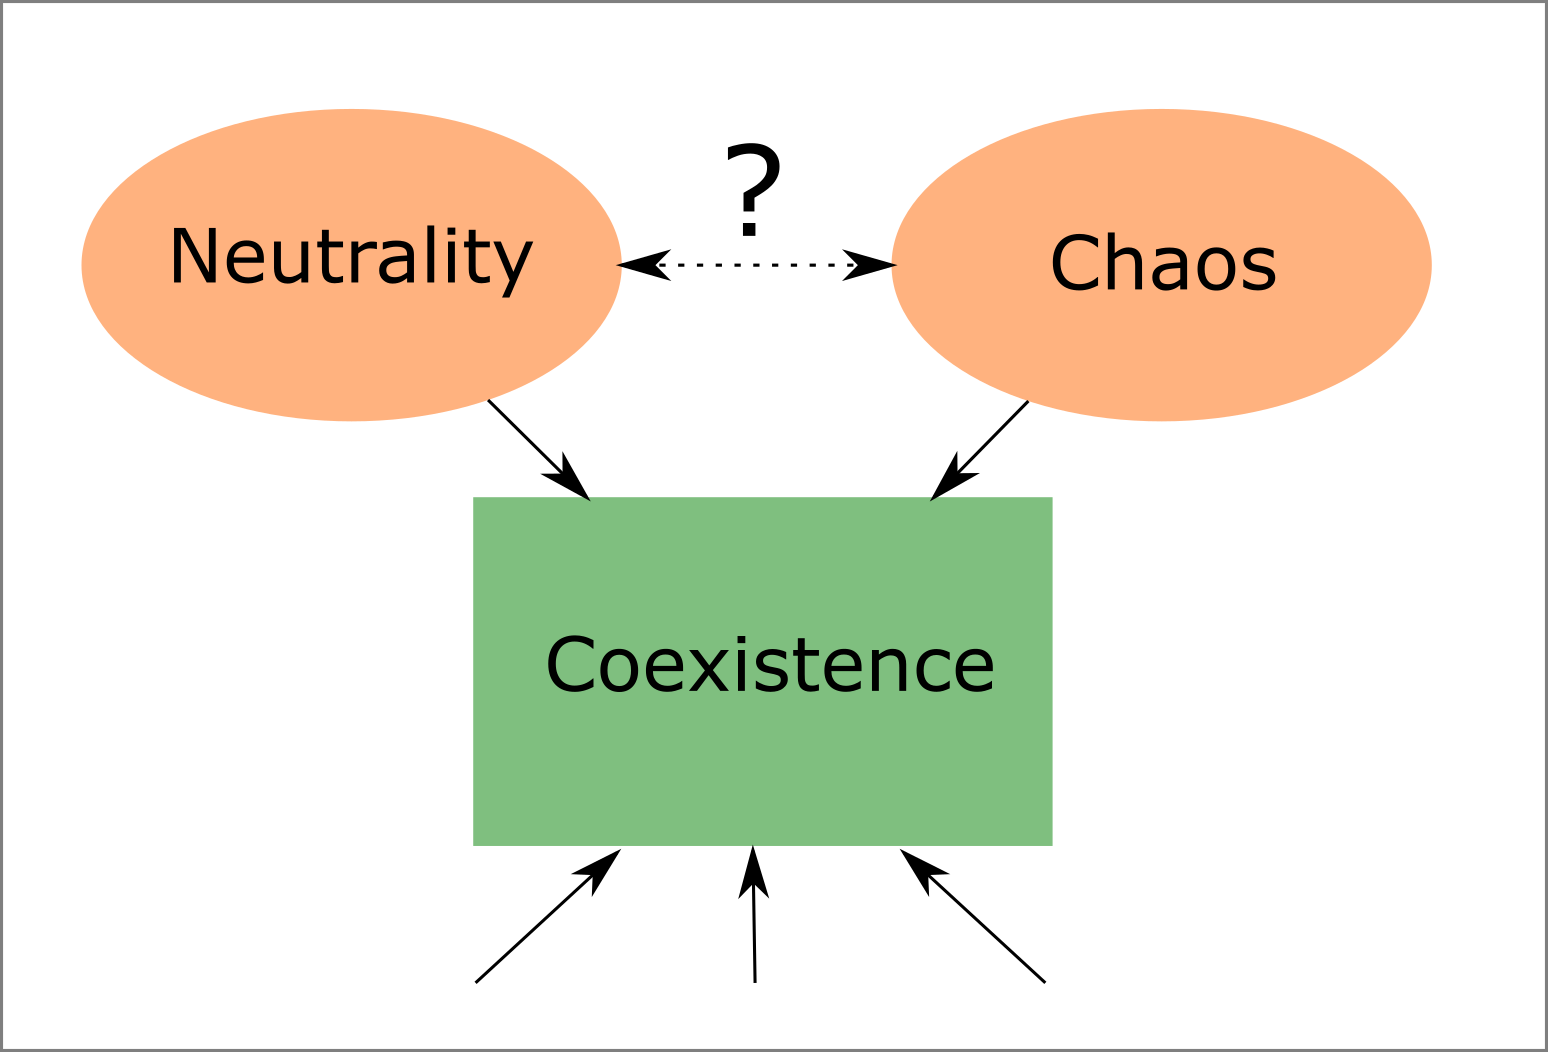
\includegraphics[width=0.5\columnwidth]{graphical_abstract.png}
	\end{center}
	\caption{In our model, neutrality and chaos are not independent explanations of coexistence.}
	\label{fig:GapInKnowledge}
\end{figure}
